\documentclass[12]{article}
\usepackage{graphicx} % this is for insert image
\usepackage{subcaption} %this is for multiple images
\usepackage[backend=bibtex, sorting=none]{biblatex} %this is needed for bibliograhy for rnw

\bibliography{ResearchProp} % name of my bibtex

% echo=F>>=
% opts_chunk$set(echo=F,message=F,warning=F)
% @

\title{Research proposal: Longitudinal effect of neighbordhood physical environment on obesity among Swedish adults}
\date{2019-02-25}
\author{Kenta Okuyama}


\usepackage{Sweave}
\begin{document}
\Sconcordance{concordance:ne_obesity.tex:ne_obesity.Rnw:%
1 16 1 1 0 126 1}

\pagenumbering{gobble} %Gobble pagenumber in title page
\maketitle
\tableofcontents
\newpage
\pagenumbering{arabic}
  
\section{Introduction} %Biggest section
\paragraph{}
Obesity can lead to serious negative health consequences, such as type 2 diabetes and cardiovascular disease, and its prevalnce has been increasing worldwide \cite{ng2014global,flegal2002prevalence}. Environmental and policy interventions are now recognized as an urgent approach to combat the global obesity epidemic \cite{gortmaker2011changing}. Although numerous research have been done on the influence of environmental features on obesity, there is no consistent evidence \cite{papas2007built,mackenbach2014obesogenic}. One of the major challenges is that majority of the studies were conducted cross-sectionally, thereby causal relationship has not been elucidated yet. \paragraph{}
A few recent studies found a significant association between neighborhood  physical environment features and obesity \cite{mason2018associations,barrientos2017neighborhood}. For example, Mason et al. found that both density of physical activity (PA) facilities and proximity to fastfood outlets were associated with adiposity in the expected direction among nation-wide adults cohort in UK. Barrientos et al. found that improvement of neighborhood enviroment in promoting both healthy eating and physical activity was related to BMI reduction among obese persons \cite{barrientos2017neighborhood}. However, despite these recent findings, the association between neighborhood physical environment and obesity are still unclear \cite{nieuwenhuijsen2018influence}. This is mainly because complex mechanism for the incidence of obesity due to numerous factors that can affect energy inbalance between diet and physical activity, such as individual socio-economic status (SES), neighborhood deprivation, and genetic risk factors (Figure 1). 
\paragraph{}
In particular, individual SES and neighborhood deprivation is most likely to modify the effect of food and PA environment on obesity. It is hypothesized from previous findings which found the greater benefitial effect of neighborhood environment on adult's obeisty or obesity related health behavior (i.e. physical activity) among high-SES group compared to low-SES group \cite{mason2018associations,owen2007neighborhood}. This could be explained that people need to have sufficient wealth in terms of money and time to benefit from neighborhoood environment, for example, whether they can afford to go to the gym. In order to put environmental and policy level action forward, equity in health needs to be addressed on whether population across different SES could benefit from interventions \cite{gortmaker2011changing}. From these backgrounds, this study consists of following two aims:


\paragraph{Aim 1}
Examine the longitudinal association between neighborhood physical environment (fast food and physical activity outlets) and obesity.
\paragraph{Aim 2}
Examine whether the association between neighborhood physical environment and obesity is confounded or modified by individual and neighborhood socio-economic status.

\begin{figure}[h!]
\centering
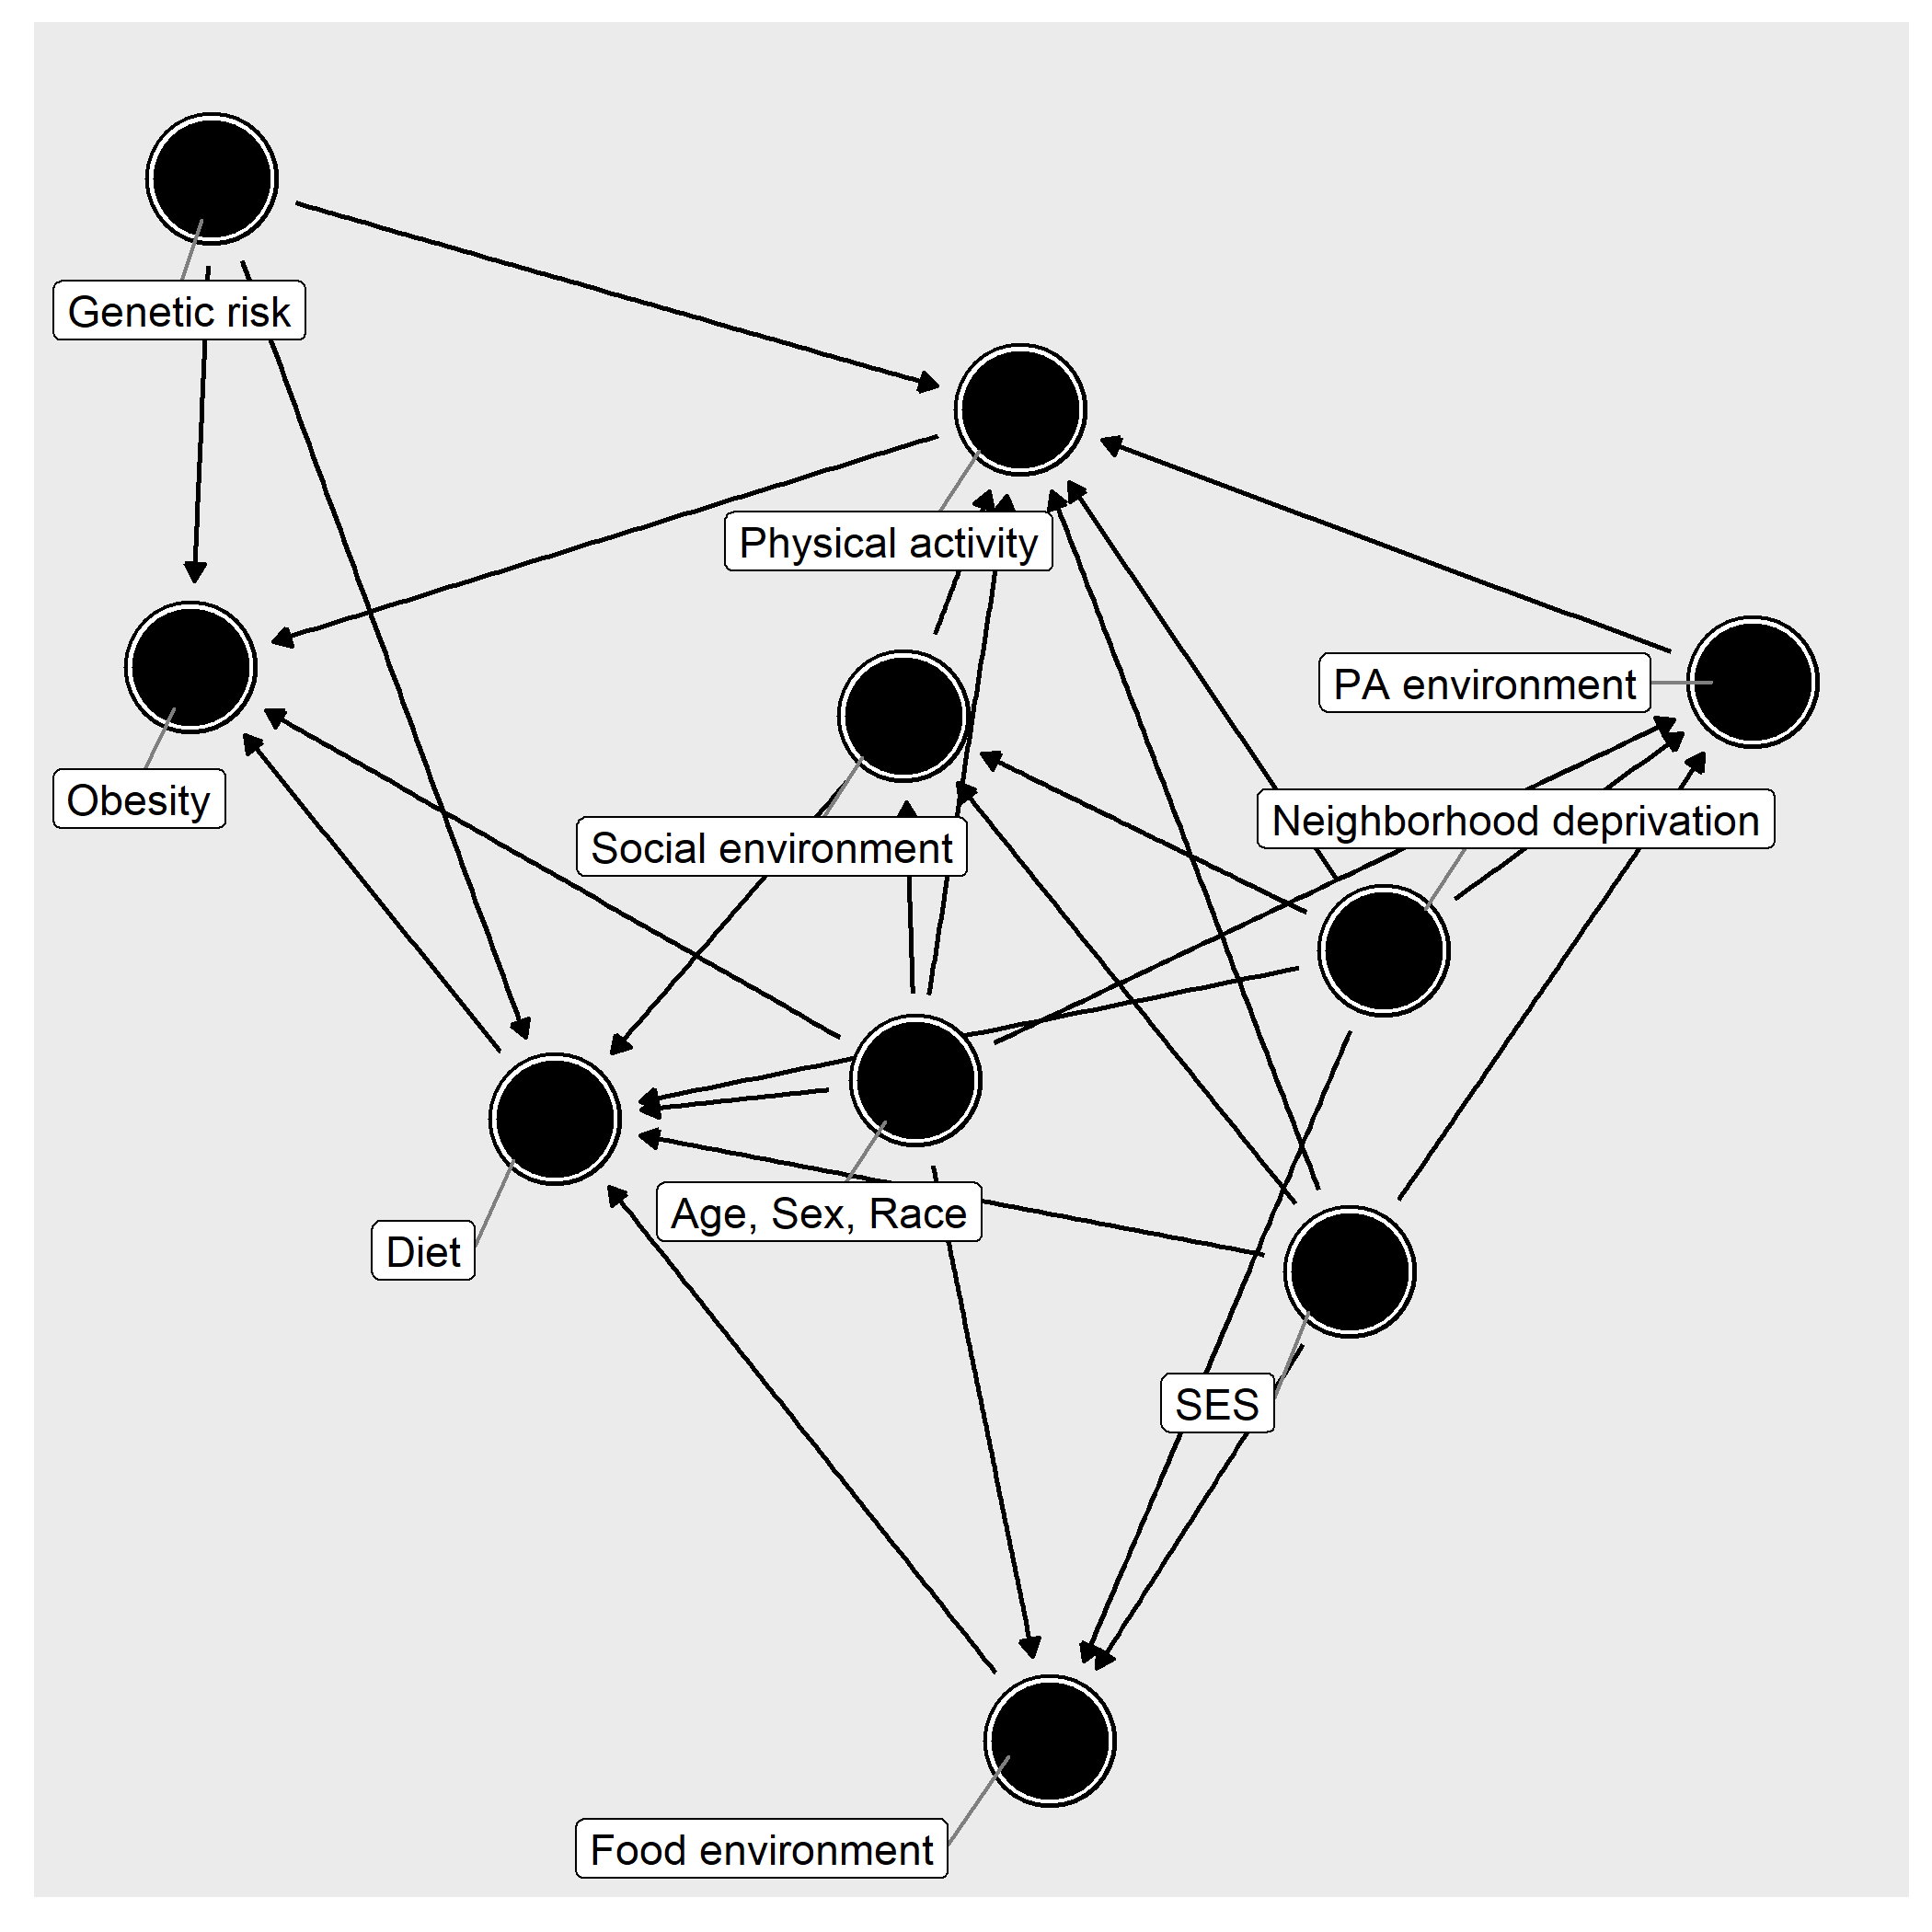
\includegraphics[width=\linewidth]{graph/dag1.png}
\caption{Directed acyclic graph for neighbrhood envrionments and obesity}
\label{fig:dag}
\end{figure}



\newpage

\section{Significance for each aim}
\paragraph{Aim 1}
Examining the casual relationship between physical environment and obesity would reinforce the evidence that emphasize the needs of environmental and policy interventions. 

\paragraph{Aim 2}
In order to implement environmental and policy intervention for obesity, equity needs
to be addressed, i.e., all individuals across socio-economic status should be able to benefit out from environment changes. Examining on how physical environment affect on obesity by different socio-economic status could put actions forward or reconsider environmental intervention for populations.

\newpage

\section{Methods}
\subsection{Aim 1: Incidence of obesity and physical envionment}
\subsubsection{Study sample}
\paragraph{} Nationwide sample of men and women age between 20 - 40 years old from a national Swedish registers. Information about women's weight, height and BMI will be obtained from the Swedish Medical Birth Resgister, which is a register of all pregnancies, prenatal care and birth records for all mothers and children in Sweden since 1973. Information about men's weight, height and BMI will be obtained from the Military Conscription Register, which includes a structured and standardized medical assessment of all Swedish men since 1969. Baseline will be set for 2005, as a ready to use neighborhood measures (i.e., density of fast food outlets, and physical activity facilities) are available at this time period. Follow-up period will be until 2015, which is the last year of available follow-up data.
\subsubsection{Outcome}
\paragraph{}    
Incidence of obesity will be identified by a hospital or out-patient diagnosis of obesity during study period. Hospital Discharge Register and Out-Patient Register will be used to collect the diagnosis of obesity, which can be linked by serial number of men and women's cohort datasets.
\subsubsection{Exposure}
\paragraph{}
Density of fast food outlets (e.g., pizzerias, and hamburger joints) and physical activity facilities (e.g., swimming pools, gyms, ski facilities) calculated by geographic information system (GIS) would be used as primary exposure variable for obesity. Neighborhood space will be defined by administrative boundary (Small Area Market Statistics (SAMS)), and counts of facilities within each boundary will be used as measures of density. Each exposure will be examined by separate models to predict the effect of each exposure on obesity (Figure 2). 

\newpage
\begin{figure}[h!]
  \centering
  \begin{subfigure}[b]{0.4\linewidth}
    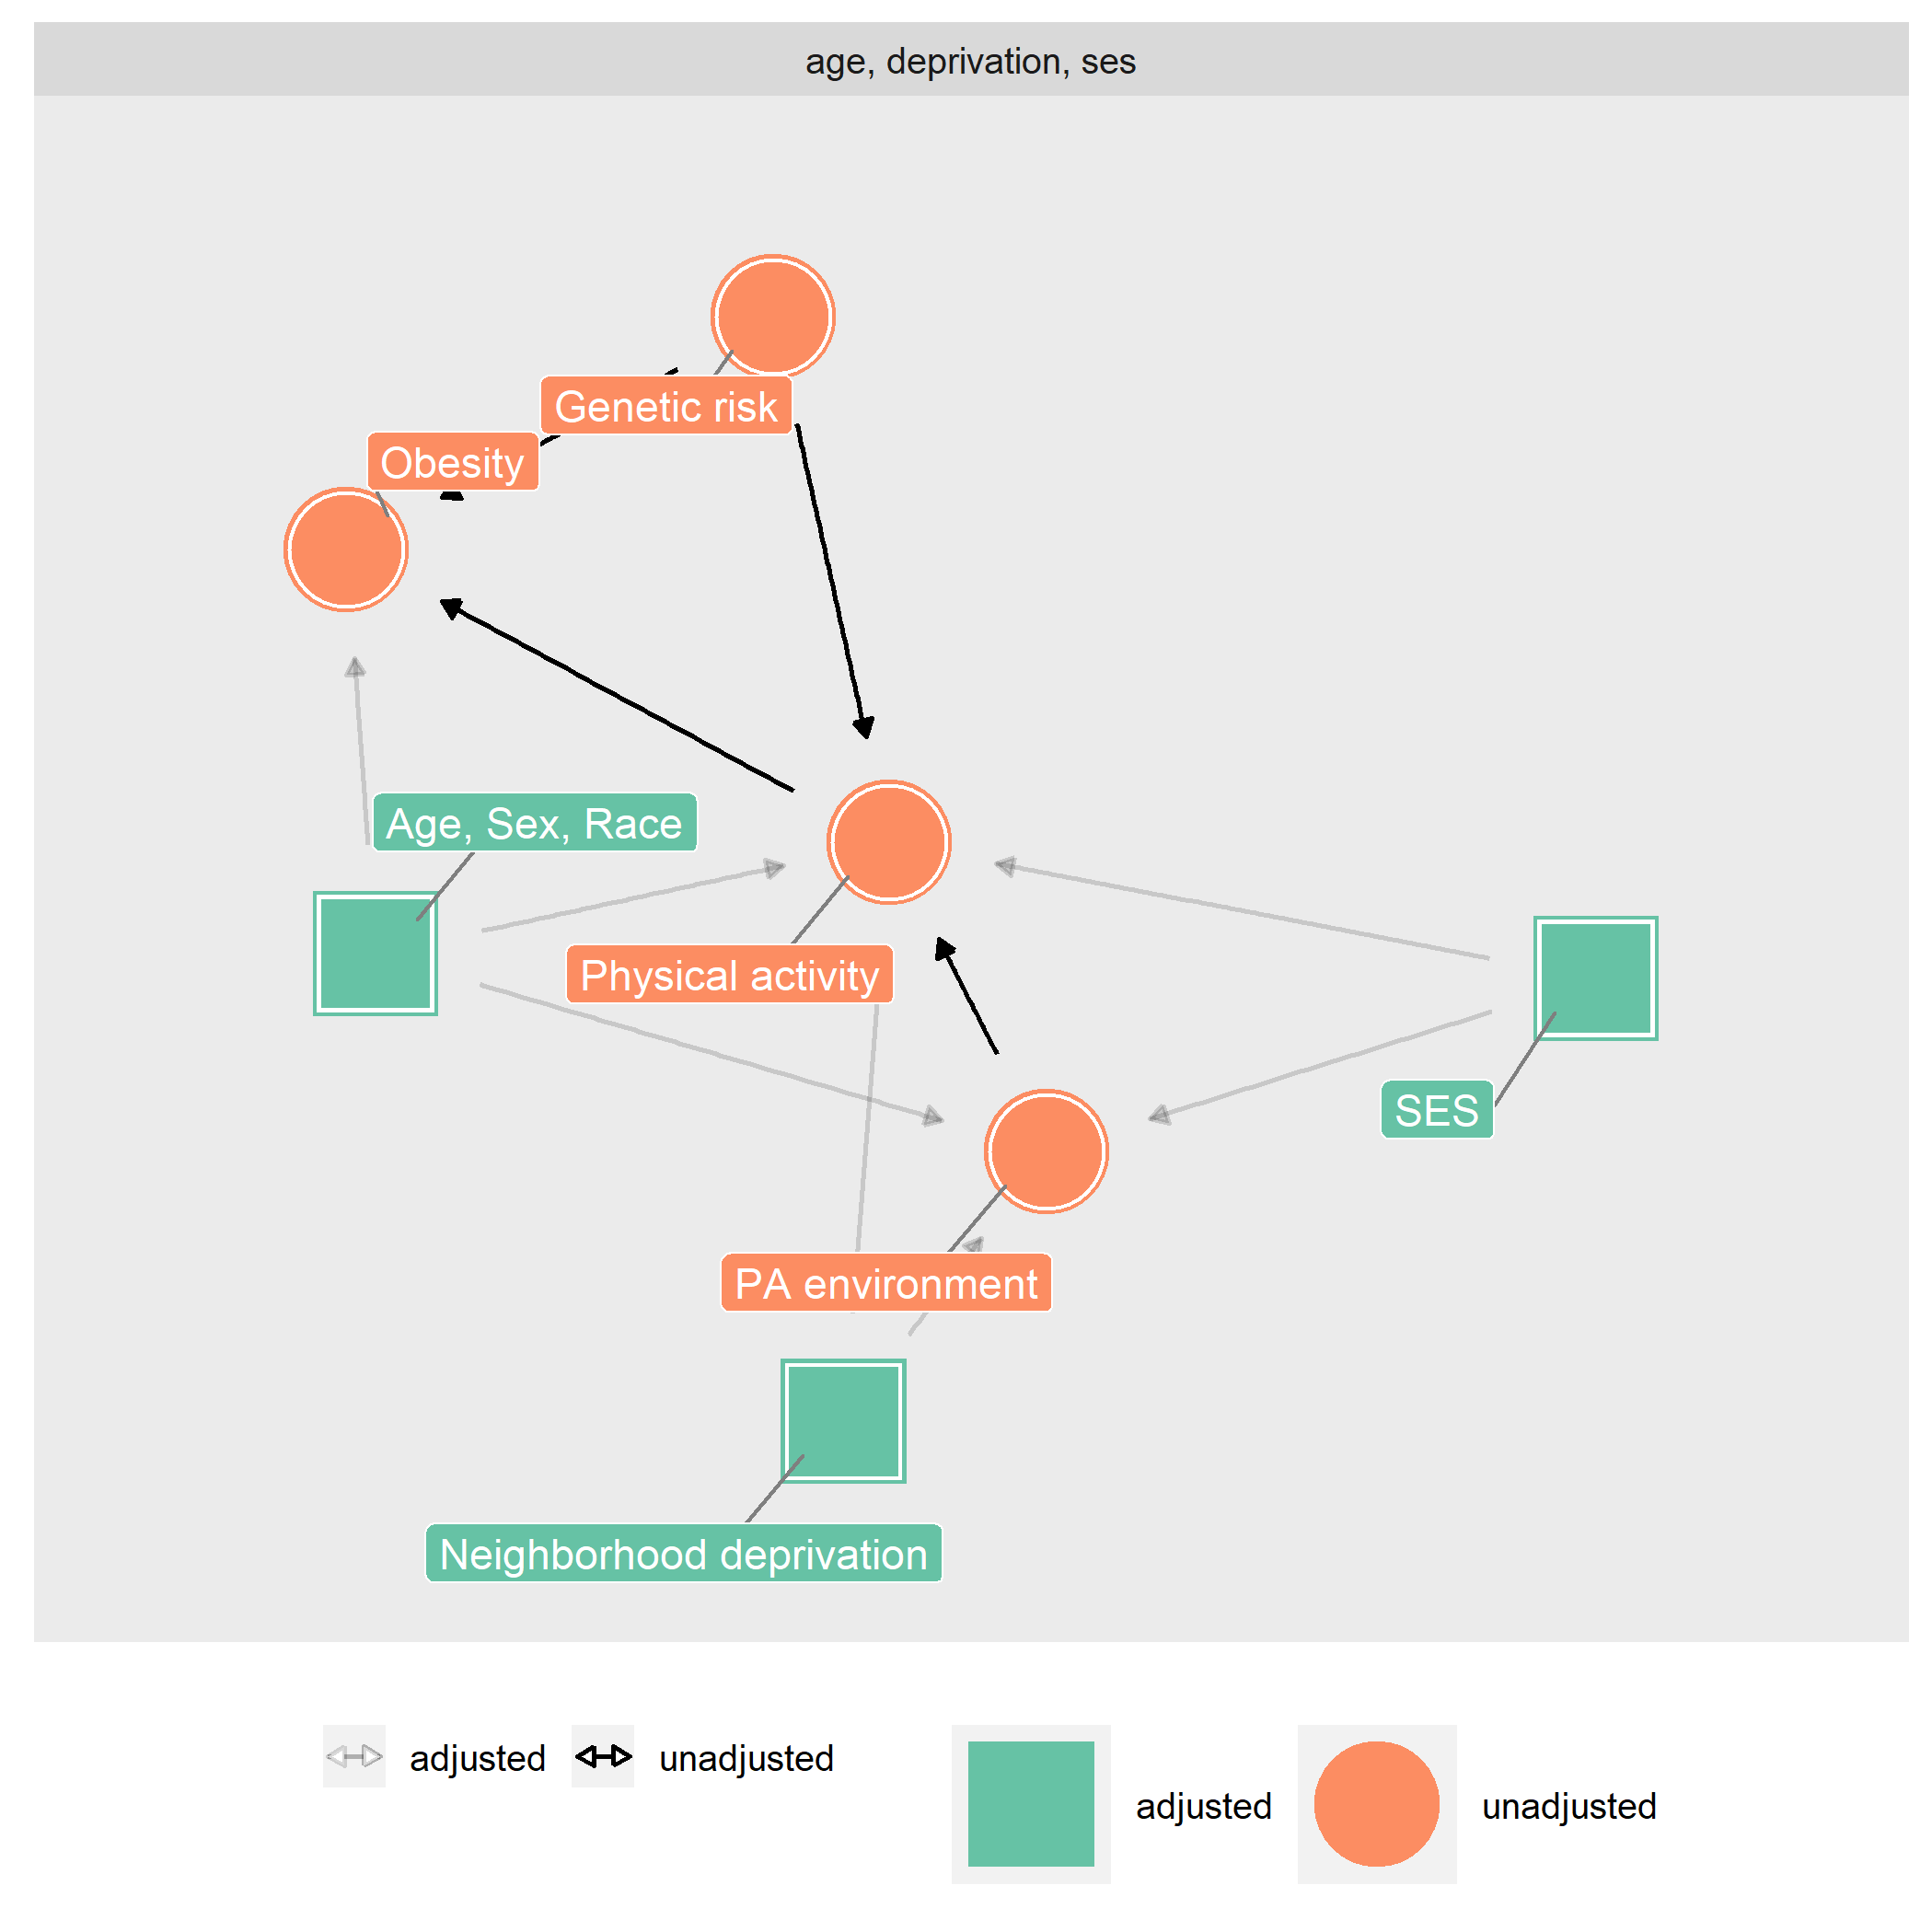
\includegraphics[width=\linewidth]{graph/dag2.png}
    \caption{PA enviornment and obesity.}
  \end{subfigure}
  \begin{subfigure}[b]{0.4\linewidth}
    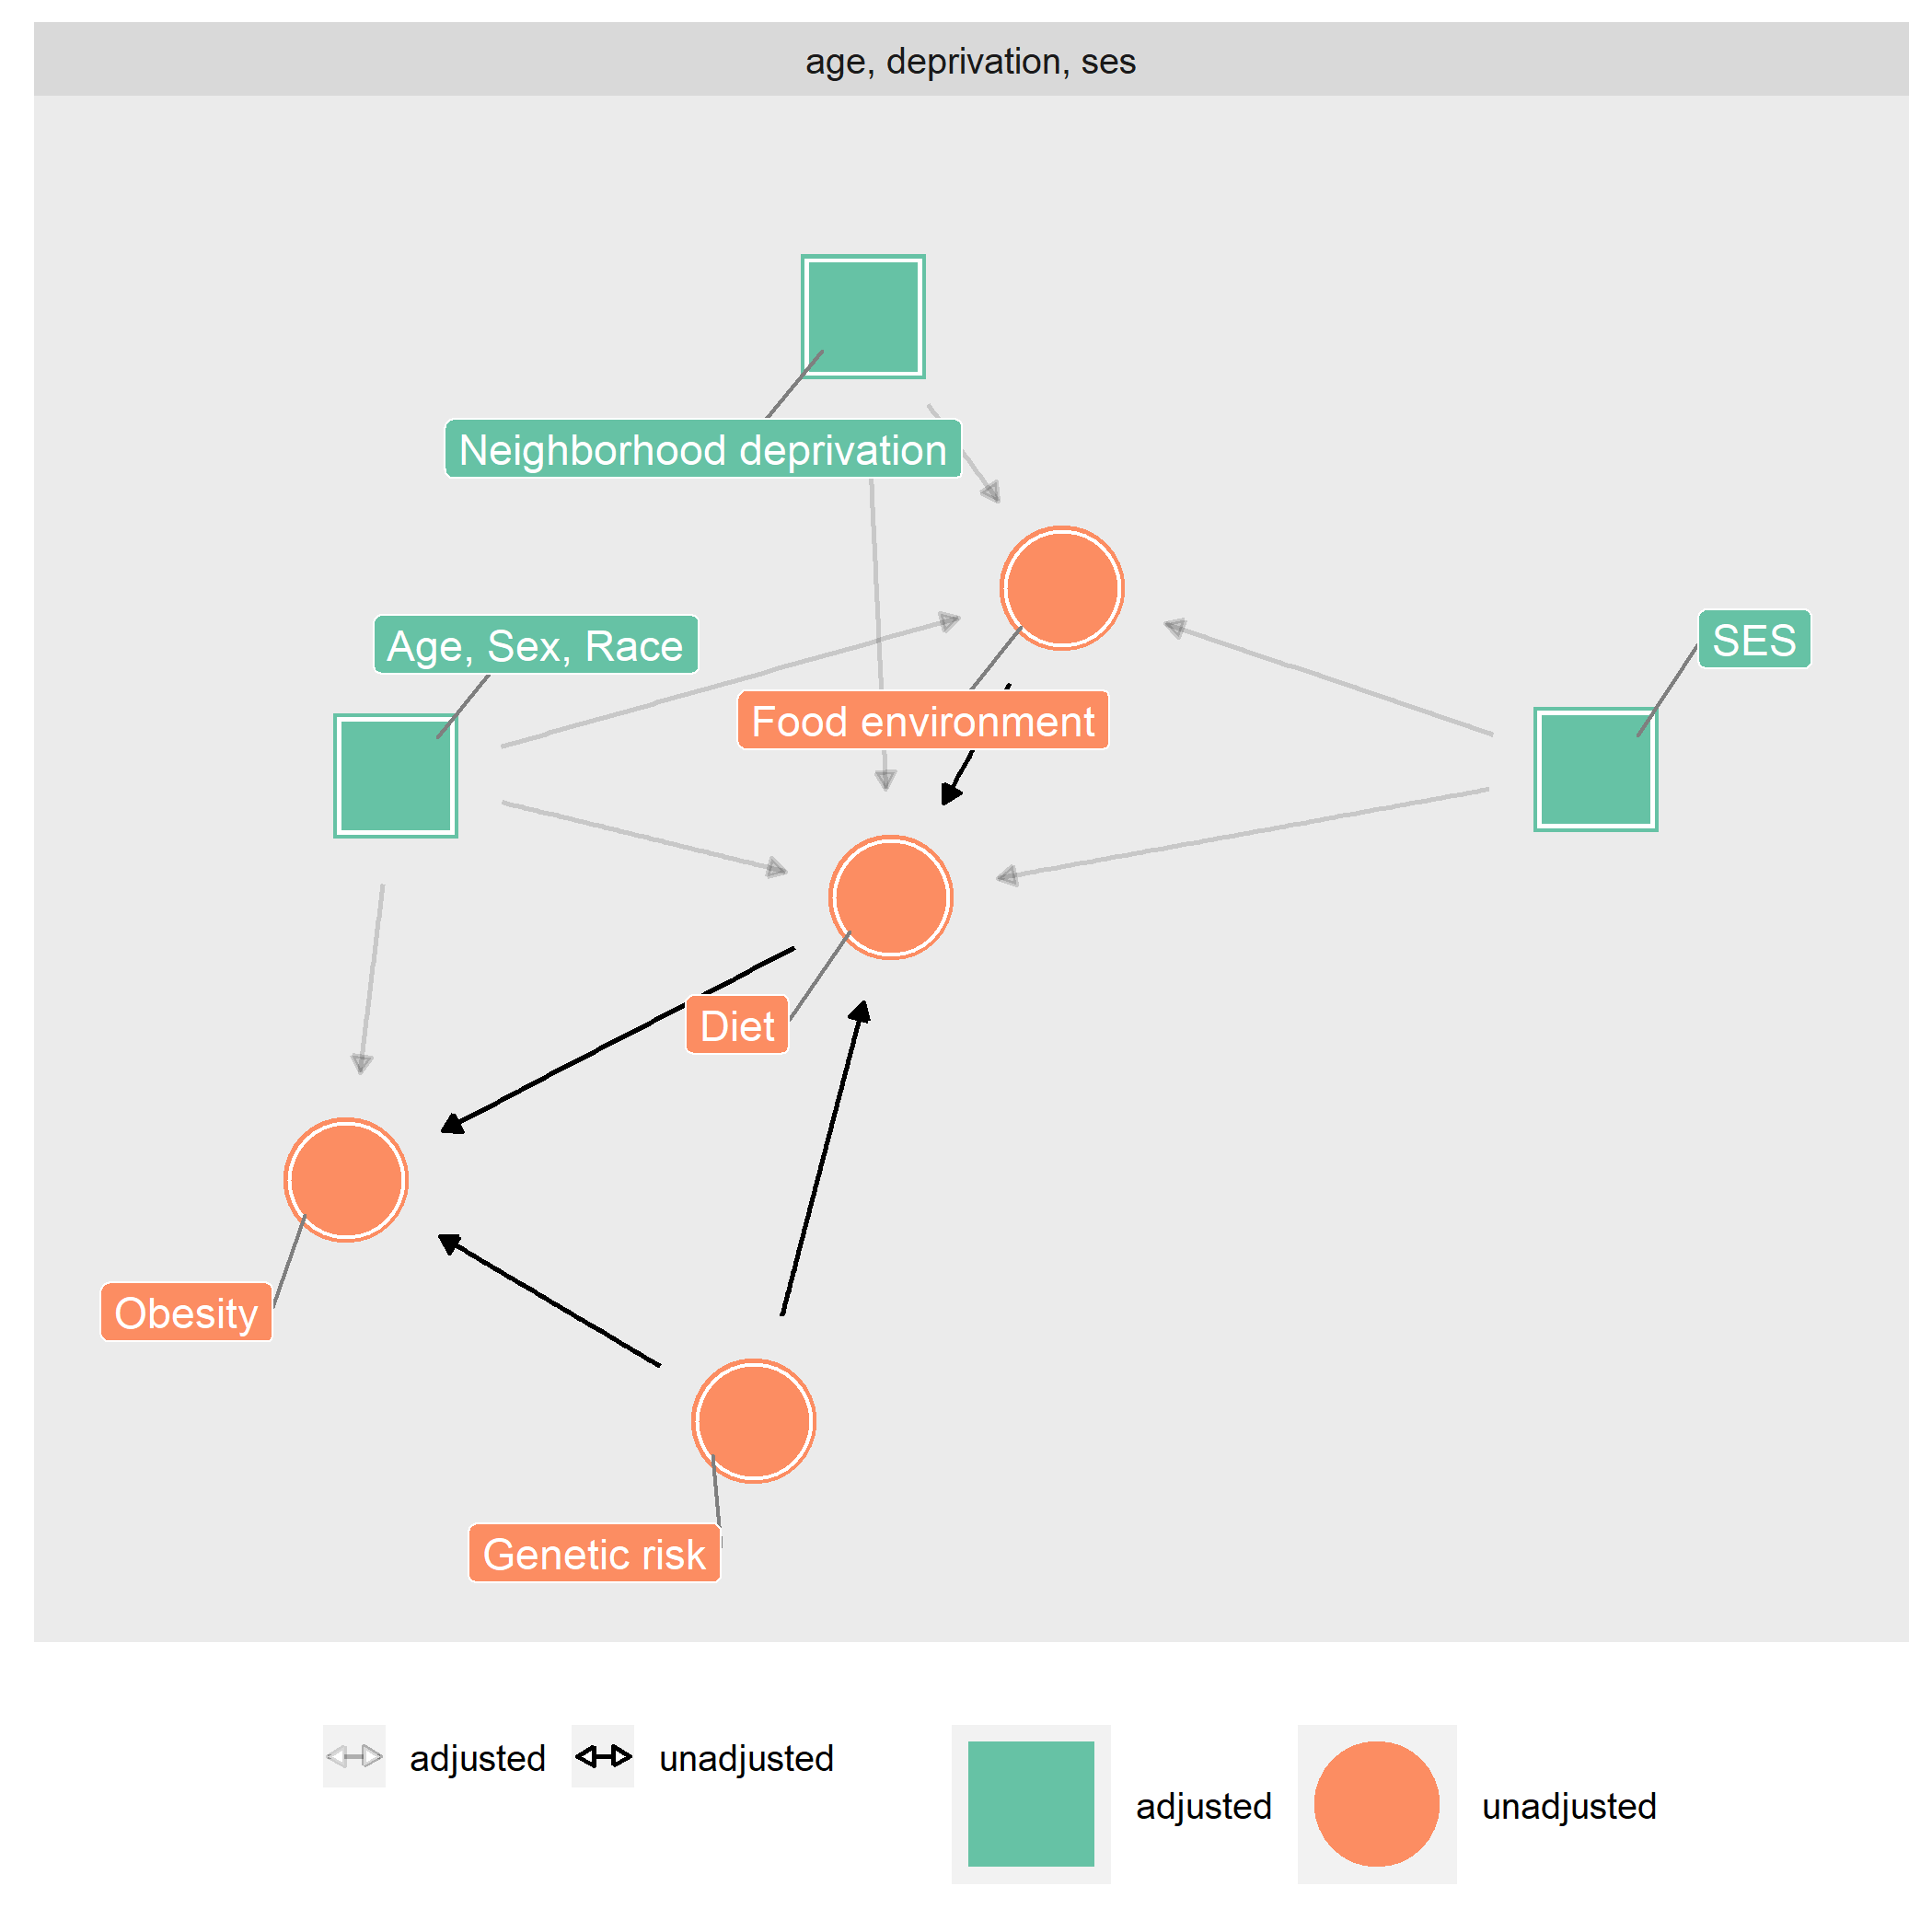
\includegraphics[width=\linewidth]{graph/dag3.png}
    \caption{Food environment and obesity.}
  \end{subfigure}
  \caption{DAG for physical activity and food environment}
  \label{fig:flight}
\end{figure}      


\subsubsection{Covariates}
\paragraph{}
Potenitial confounding variables and effect modifiers, i.e., age, gender, BMI at baseline, immigration status, family income, educational attainment, occupation, and neighborhood deprivation will be controlled (Table 1).  

\begin{table}[h!]
		    \caption{Description of variables to be analyzed}
		    \label{table:aim1}
		      \centering
		      \begin{tabular}{ c l p{5cm} }
			    \hline
			    Type & Name & Description\\
			    \hline \hline
			    Outcome & Obesity & Incidence of obesity identified from the Hospital Discharge Register and Out-Patient Register.\\
			    Exposure & Food environment & Density of fastfood outlets (e.g., pizzerias, and hamburger joints).\\
			             & Physical activity environment &  Density of physical activity facilities (e.g., swimming pools, gyms, ski facilities)\cite{kawakami2011health}.\\
			    Covariates & Basic characteristics & Age, gender, baseline BMI, and immigration status. \\
			               & Socio-economic status & Education, occupation, and income.\\
				            & Neighborhood deprivation & Neighborhood deprivation index measured by poverty level \cite{kawakami2011differences}.\\
          \hline
			    \end{tabular}
			  \end{table}
\subsubsection{Statistical analysis}
\paragraph{}
The cumulative rate of obesity will be calculated for the total study population. Multilevel logistic regression will be applied.
	    


\subsection{Aim 2: Interaction effect of physial environment and individual SES and neighborhood deprivation on obesity}
\subsubsection{Sensitivity analysis}
\paragraph{}
Conduct stratified analysis by individal SES and neighborhood deprivation.  

\section{Limitations and Future studies}
\paragraph{}
One of the major limitations of this study is that we cannot take longitudinal environmental change into accout. This is often a major challenge in neighborhood studies as neighborhood environments are most likely to change over time. As another limitation, we cannot identify whether individuals stayed in the same neighborhood over time. Both makes it difficult to elucidate causal relationship between neighborhood environment and population health. Future studies need to consider these limitations and conduct more robust analysis. If there is a enviornmental components which have significantly changed over time, it could be an intrest of exploration with longitudinal population health statuses. In Shimane Japan, for example, the highway has been connecting between the east and west part of Shmane region over this past 10 years, and this is the largest environmental change (Figure 3).

\begin{figure}[h!]
\centering
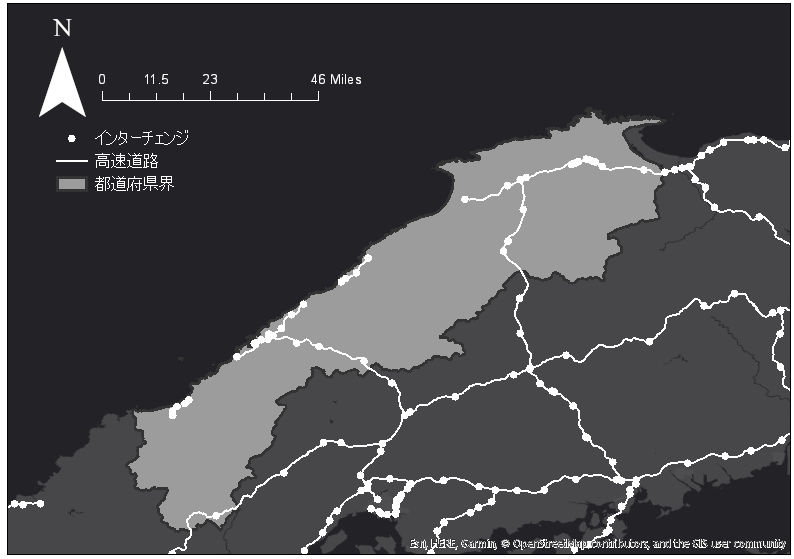
\includegraphics[width=10cm,height=10cm,keepaspectratio]{graph/highway.jpg}
\caption{Highway connecting the east and west of Shimane, Japan}
\label{fig:highway}
\end{figure}

\newpage
\section{Litterature review}
\subsection{Physical environments}
\paragraph{}
Originally, physical environments have been identified as one of the important determinants on human behaviors based on ecological and socio-ecological model which had evlolved in the late 1900s \cite{mcleroy1988ecological,sallis1998environmental}. Ecological model specifies levels of influence on behavior, from individual, institutional, community, enviornmental, and policy factors \cite{mcleroy1988ecological}. Although there were growing recognitions for the potential effect of environment and policy interventions in the population level, few interventons have been applied to the control of chronic diseases as of late 1900s \cite{schmid1995policy}. It is often challenging to implement environment and policy level interventions as it requires substential investiments and collaborations in various sectors (e.g.health, transportation,and urban planning).

Numerous efforts have been made to put it foward by Sallis et al. specific to physical activity to stimulate more research in this field in order to accumulate sufficient evidences for enviornment and policy changes \cite{sallis1998environmental}. 
\paragraph{}
Since early 2000s, neighborhood research have been accelerated, especially because technologies made it possible to objectively assess physical environment, i.e. geographic information system (GIS). GIS, which used to be utilized in the field of geographics and urban planning to evaluate geography and structure of cities by numerical data, had been incorporated into health field  \cite{frank2005linking}. Collaboration with urban planning and health fields put emphasis on the need of creating "walkable" neighborhoods by focussing on human-made built environments, which had been already recognized for safety perspective, such as Smart Growth America \cite{smartgrowth}.
In several places in the US, environmental interventions to promote healthy behavior had been implemented, such as building public transit or securing walking and cycling infrastructures \cite{brown2015transit,macdonald2010effect}. Although the effects of these interventions have been examined by study design of natural experiments, there are no robust evidences on whether it is effective for reducing the risk of obesity in the population level \cite{tseng2018effectiveness}. Lack of evidences for the association between physical environment and obesity remains as a barrier for implementing enviornmental interventions. 

\newpage

\printbibliography
\end{document}
